\documentclass{article}


% if you need to pass options to natbib, use, e.g.:
    % \PassOptionsToPackage{numbers, compress}{natbib}
% before loading neurips_2022


% ready for submission
% \usepackage{neurips_2022}


% to compile a preprint version, e.g., for submission to arXiv, add add the
% [preprint] option:
\usepackage[preprint]{neurips_2022}


% to compile a camera-ready version, add the [final] option, e.g.:
% \usepackage[final]{neurips_2022}


% to avoid loading the natbib package, add option nonatbib:
% \usepackage[nonatbib]{neurips_2022}


\usepackage[utf8]{inputenc} % allow utf-8 input
\usepackage[T1]{fontenc}    % use 8-bit T1 fonts
\usepackage{hyperref}       % hyperlinks
\usepackage{url}            % simple URL typesetting
\usepackage{booktabs}       % professional-quality tables
\usepackage{amsfonts}       % blackboard math symbols
\usepackage{nicefrac}       % compact symbols for 1/2, etc.
\usepackage{microtype}      % microtypography
\usepackage{xcolor}         % colors

\usepackage{graphicx}
\graphicspath{ {./figures/} }


\title{Video Frame Prediction}


% The \author macro works with any number of authors. There are two commands
% used to separate the names and addresses of multiple authors: \And and \AND.
%
% Using \And between authors leaves it to LaTeX to determine where to break the
% lines. Using \AND forces a line break at that point. So, if LaTeX puts 3 of 4
% authors names on the first line, and the last on the second line, try using
% \AND instead of \And before the third author name.


\author{%
  Swapnil Sharma\thanks{\url{https://swappysh.github.io}} \\
  \texttt{swapnil.sh@nyu.edu} \\
  % examples of more authors
  \And
  Nikita Anand \\
  \texttt{email} \\
  \And
  Rishika Pabba \\
  \texttt{email} \\
  % \AND
  % Coauthor \\
  % Affiliation \\
  % Address \\
  % \texttt{email} \\
  % \And
  % Coauthor \\
  % Affiliation \\
  % Address \\
  % \texttt{email} \\
  % \And
  % Coauthor \\
  % Affiliation \\
  % Address \\
  % \texttt{email} \\
}


\begin{document}


\maketitle


\begin{abstract}
  This abstract details an attempt to solve a video frame prediction task by utilizing various 
models and techniques, including ConvLSTM, Segformer, and AutoEncoders for semantic segmentation 
mask, ConvLSTM in an auto-regressive manner, ConvBiLSTM in a non-auto regressive manner by 
predicting all frames at once, and ultimately settling on VPTR Non Auto Regressive due to its 
convergence on a subset of data. The authors encountered significant challenges with training 
time and memory constraints, and attempted to address these issues by using mixed precision 
training and unsuccessfully attempting to train on multiple GPUs using PyTorch Distributed Data 
Parallel.

The ResNet AutoEncoders proved to be the most effective for the semantic segmentation mask with 
an impressive accuracy of 0.993 on the validation set. The VPTR model achieved a decent accuracy 
of 0.9 on a subset of the data for video frame prediction. Although the model was unable to 
converge on the whole dataset due to time and memory constraints, the authors believe that with 
more time and resources, they would have achieved better accuracy in predicting future frames.
\end{abstract}

\section{Introduction}
In recent years, predicting future frames in videos has become a challenging task that has 
attracted extensive research. This task has numerous applications, including video compression, 
editing, and surveillance. This report documents an attempt to solve a video frame prediction 
task presented by the NYU Deep Learning Course, which required predicting the semantic 
segmentation mask of the 22\textsuperscript{nd} frame of a video based on the initial 11 
frames.

The videos used in this project featured simple 3D shapes that interacted with each other 
based on basic physics principles. Each object in the videos was uniquely identified by a 
combination of three attributes: shape (cube, sphere, or cylinder), material (metal or rubber), 
and color (gray, red, blue, green, brown, cyan, purple, or yellow). No identical objects 
appeared in a single video.

To address the challenges of semantic segmentation mask translation and future frame prediction, 
we explored several approaches, including ConvLSTM, Segformer, ResNet AutoEncoders, convBiLSTM, 
and non-autoregressive VPTR. The ResNet AutoEncoders achieved the best results for the semantic 
segmentation mask translation task with an accuracy of 0.993 on the validation set. For the 
future frame prediction task, we achieved the best performance on a subset of the dataset using 
the VPTR model, although we were unable to converge the model on the entire dataset due to 
time and memory constraints.

\section{Related Work}
Most state-of-the-art (SOTA) models for video frame prediction use ConvLSTM-based AutoEncoders. 
These models were initially developed for predicting precipitation nowcasting, as introduced by 
\citet{Shi2015ConvolutionalLN}. They have been later utilized for video prediction task, including 
\citet{Finn2016UnsupervisedLF}, \citet{Lotter2016DeepPC}, \citet{Xu2016EndtoEndLO}, 
\citet{Ballas2015DelvingDI}. According to \citet{Jing2019SelfSupervisedVF}, these models also 
work with self-supervised tasks.

Although the ConvLSTM-based models are flexible and efficient, they are generally slow due to 
recurrent prediction. To address this issue, standard CNNs or 3D CNNs and VAE-based methods 
have been proposed, such as those by \citet{Mathieu2015DeepMV} and 
\citet{Babaeizadeh2017StochasticVV}.

State-of-the-art models commonly rely on complex ConvLSTM models integrating attention mechanisms 
or memory-augmented modules. For instance, the Long-term Motion Context Memory model by 
\citet{Lee2021VideoPR} stores long-term motion context through a novel memory alignment learning, 
and the motion information is recalled during the test to facilitate long-term prediction. 
\citet{Chang2021MAUAM} proposed an attention-based motion-aware unit to increase the temporal 
receptive field of RNNs.

Almost all the state-of-the-art (SOTA) VFFP models are based on ConvLSTMs, i.e. convolutional 
short-term memory networks,which are efficient and powerful. Nevertheless as per \citet{Ye2022VPTRET}, 
they suffer from some inherent problems of recurrent neural networks(RNNs), such as slow training 
and inference speed, error accumulation during inference, gradient vanishing, and predicted 
frames quality degradation. Researchers keep improving the performance by developing more and 
more sophisticated ConvLSTM-based models. 

With the introduction of transformers, they have also been applied in the Vision domain, 
including video frame prediction. The ConvTransformer model by \citet{Liu2020ConvTransformerAC} 
follows the architecture of DETR introduced in \citet{Meinhardt2021TrackFormerMT}, a classical 
neural machine translation (NMT) Transformer architecture. DETR also inspired the development 
of the VPTR-NAR model by \citet{Ye2022VPTRET}, a non-autoregressive model for video frame 
prediction.

\section{Methodology}
\subsection{Semantic Segmentation Mask}
We settled on ResNet AutoEncoders to solve the semantic segmentation mask translation task after 
exploring multiple approaches. ResNet, a CNN architecture with skip connections, was used to 
avoid vanishing gradients. AutoEncoders, a type of neural network for dimensionality reduction,
were employed to learn representations of the input using the encoder and to construct a 
semantic segmentation mask from the learned representation using the decoder. To simplify 
training, we removed any skip connections between the encoder and decoder layers, as suggested 
by \citet{Ye2022VPTRET}.

The encoder was composed of nine ResNet blocks, each with two convolutional layers. The decoder 
contained three deconvolutional layers with one filter and a sigmoid activation function at the 
end to produce a semantic segmentation mask with a channel dimension of 49. We used Mean Square 
Error Loss and the Adam optimizer with a learning rate of 0.0002 to train the model. Due to 
memory constraints, we trained the model with a batch size of 1 for 100 epochs. We trained the 
model on 1000 labeled videos and validated it on another 1000 labeled videos. The model took 
approximately 16 hours to train on a single GPU.

\begin{figure}
  \centering
  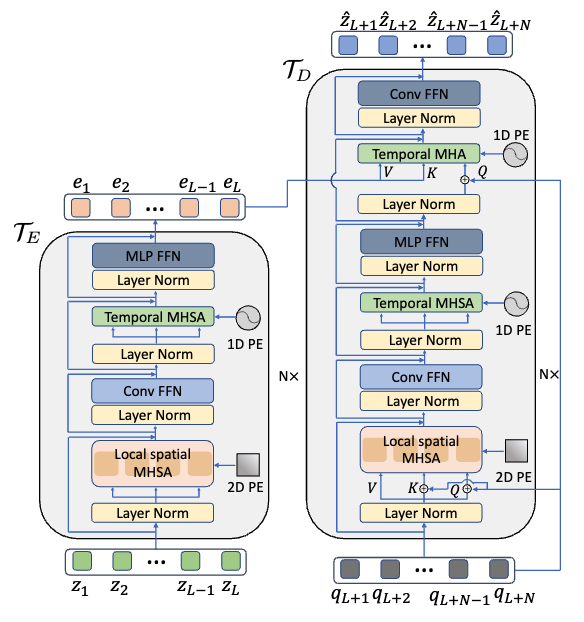
\includegraphics[scale=0.25]{VPTR_arc.png}
  \caption{VPTR NAR model architecture}
  \label{fig:architecture}
\end{figure}

\subsection{Future Frame Prediction}
In the second task of predicting future frames, we experimented with various models, including 
ConvLSTM, convBiLSTM, and VPTR. Ultimately, we chose VPTR-NAR as it was the most recent and 
state-of-the-art model for video frame prediction. \citet{Ye2022VPTRET} has two approaches one 
autoregressive and another non-autoregressive. As per their results they conculded that
NAR works better and hence we decided to use NAR. NAR utilizes a transformer encoder and a 
transformer decoder in its architecture.

The architecture of VPTR is illustrated in Figure \ref{fig:architecture}. The left part of the 
figure, denoted as $\mathcal{T}_E$, represents the encoder, which encodes all past frame 
features $z_t$ ($t \in [1, L]$) into memory representations $e_t$ ($t \in [1, L]$). The 
architecture of $\mathcal{T}_E$ comprises multiple VidHRFormer blocks, each of which contains a 
multi-head self-attention layer, a feed-forward layer, and a layer normalization layer.

On the right part of the figure, denoted as $\mathcal{T}_D$, the decoder is illustrated. It 
includes two additional layers compared to $\mathcal{T}_E$: a temporal multi-head attention 
(MHA) layer and an output convolutional feed-forward network (Conv FFN) layer. The Temporal MHA 
layer is also known as the encoder-decoder attention layer, which takes the memories as value 
and key, and queries derived from the future frame query sequence ${q_{L+1}, \cdots, q_{L+N} }$.

\section{Dataset}
The dataset consists of 13,000 unlabeled videos, 2,000 labeled videos and 1000 test videos. 
The labeled videos are further divided into 1,000 training videos and 1,000 validation videos. 
Labeled and unlabeled videos have 22 frames each and the test videos have 11 frames each.
Labeled videos also have the semantic segmentation mask for all the frames. All the frames and 
the semantic segmentation masks are of size $160 \times 240$.

We created two different datasets for the two tasks. For the first task of semantic
segmentation mask translation, we used the labeled videos and constructed a dataset consisting
of frames with their corresponding semantic segmentation masks. For the second task of future
frame prediction, we utilized only the unlabeled videos containing 11 frames each along with
the corresponding 11 future frames to construct the dataset.

\begin{figure}
  \centering
  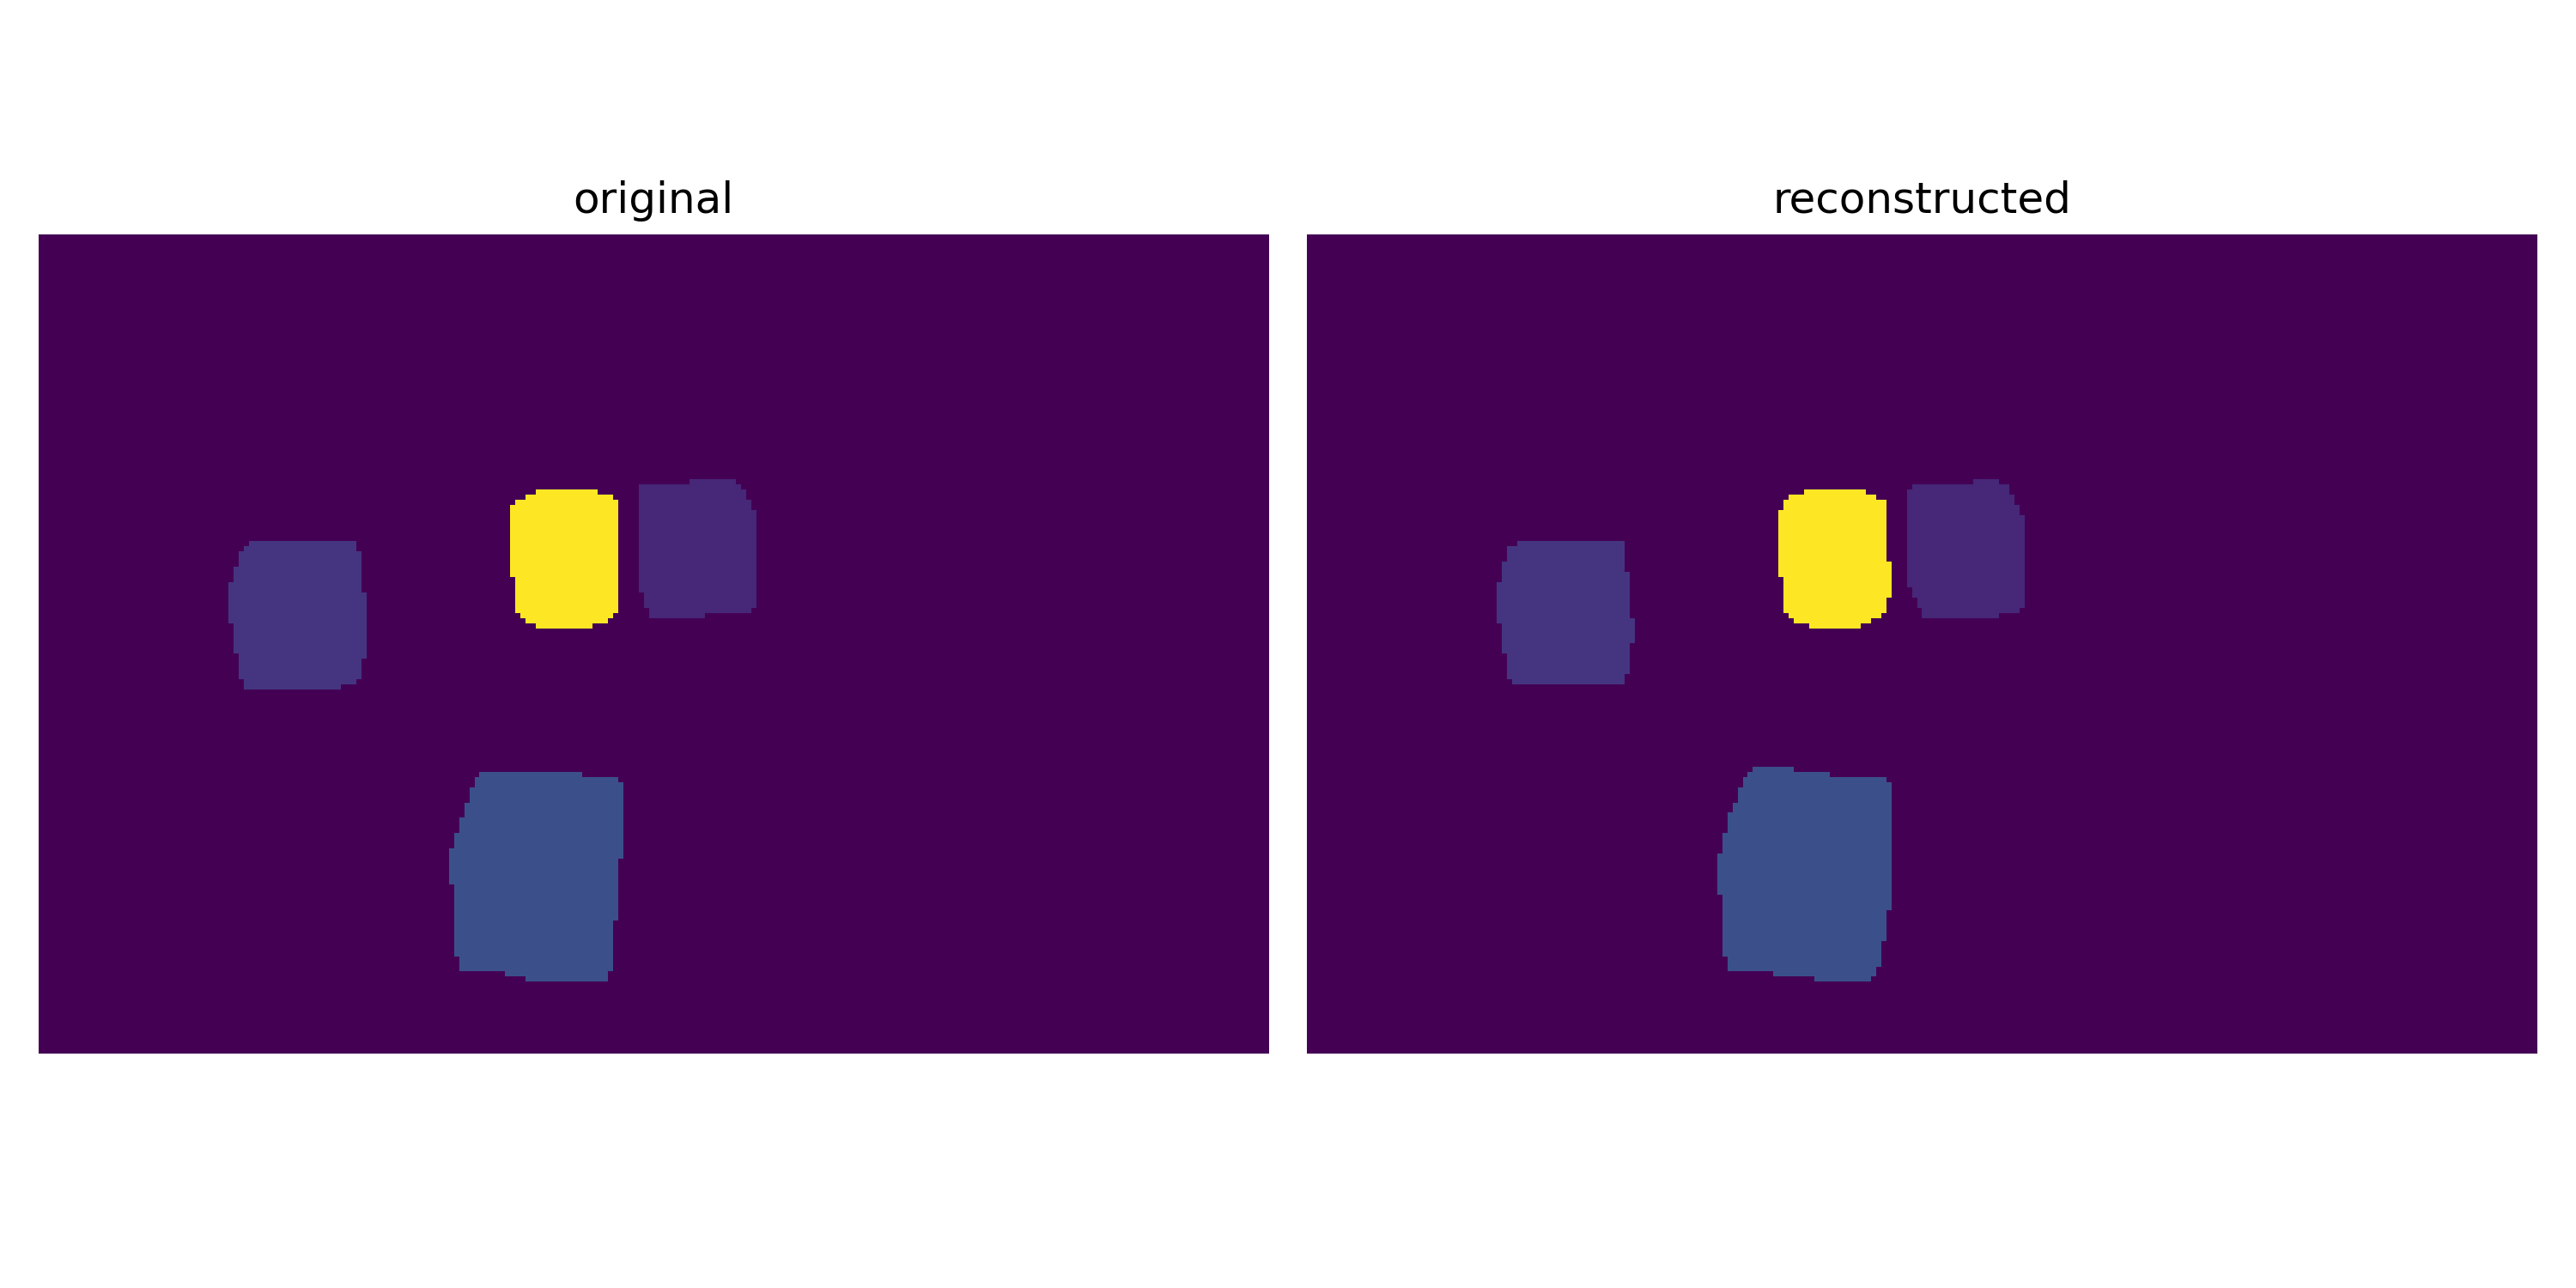
\includegraphics[scale=0.25]{reconstructed.png}
  \caption{Reconstructed semantic segmentation mask}
  \label{fig:reconstructed}
\end{figure}

\begin{figure}
  \centering
  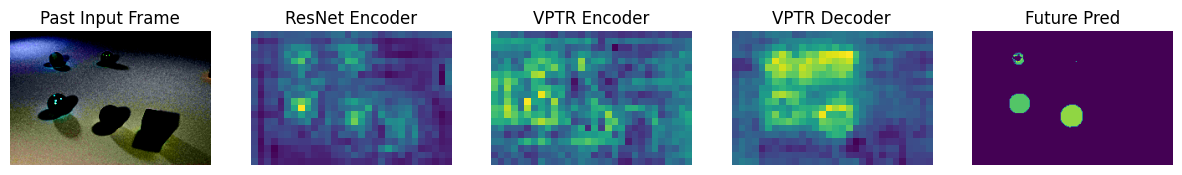
\includegraphics[scale=0.3]{VPTR_pipeline.png}
  \caption{Frame prediction pipeline}
  \label{fig:pipeline}
\end{figure}

\begin{figure}
  \centering
  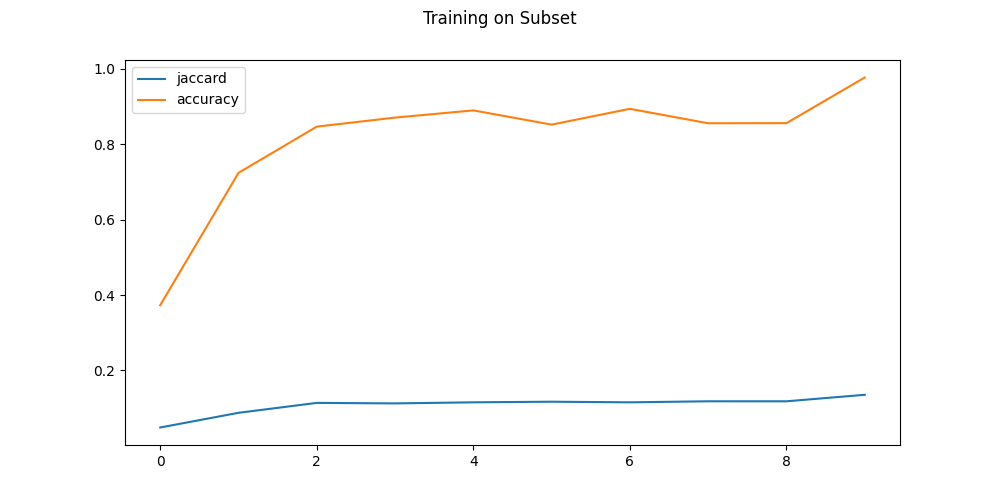
\includegraphics[scale=0.3]{subset.png}
  \caption{Training on subset of frames}
  \label{fig:subset}
\end{figure}


\section{Results}
Our experiments started with predicting the semantic segmentation mask of the frames given
normalized images of the frames. We tested ConvLSTM, Segformer, and ResNet AutoEncoders. Both
ConvLSTM and Segformer showed good performance, achieving a decent accuracy of 0.93. However,
ResNet AutoEncoders outperformed them, achieving a startling accuracy of 0.993 on the validation
set. Figure \ref{fig:reconstructed} shows the reconstructed semantic segmentation mask for a
frame predicted by the ResNet AutoEncoders.

For the second task of future frame prediction, we attempted to use ConvLSTM, convBiLSTM, and
VPTR. However, we found that ConvLSTM and ConvBiLSTM were not effective, as they took a long time
to converge and yielded poor-quality results. VPTR showed promising results on a subset of the
data, as can be seen in Figure \ref{fig:subset}. However, we encountered memory constraints and
were unable to train the model on the entire dataset, unable to exceed a batch size of 1. We
explored using DataParallel and DataDistributedParallel to utilize multiple GPUs, but due to
tight memory constraints, the overhead of using these libraries was too great. We were able to
reduce per-epoch runtime from 6 hours to 3 hours by utilizing AMP (Automatic Mixed Precision)
and Gradient Scaling.

Figure \ref{fig:pipeline} shows the zeroth input, intermediate feature, and zeroth output of the
VPTR-NAR model. From the ResNet Encoder feature, it can be observed that the model is able to see
the objects in the frame. However, it is difficult to discern what the VPTR Encoder is learning,
as it is supposed to be the attention layer output for each frame. The VPTR Decoder output shows
that it vaguely understands where the objects should be, and then produces the future frame
prediction.

\section{Conclusion}
In summary, we were able to achieve a very high accuracy of 0.993 on the semantic segmentation
mask translation task using ResNet AutoEncoders. We achieved a decent accuracy of 0.9 on the
future frame prediction task on a subset of the data, but the model did not perform as well on
the test set, achieving only a 0.03 Jaccard score. Due to time and memory constraints, we were
not able to converge the model on the entire dataset. With additional resources and time, we
believe that we would have been able to achieve a better accuracy on the future frame prediction
task.

\bibliographystyle{plainnat}
\bibliography{references}

\end{document}